\documentclass{article}


\usepackage{arxiv}

\usepackage[utf8]{inputenc} % allow utf-8 input
\usepackage[T1]{fontenc}    % use 8-bit T1 fonts
\usepackage{hyperref}       % hyperlinks
\usepackage{url}            % simple URL typesetting
\usepackage{booktabs}       % professional-quality tables
\usepackage{amsfonts}       % blackboard math symbols
\usepackage{nicefrac}       % compact symbols for 1/2, etc.
\usepackage{microtype}      % microtypography
\usepackage{lipsum}
\usepackage{fancyhdr}       % header
\usepackage{graphicx}       % graphics
\graphicspath{{media/}}     % organize your images and other figures under media/ folder

\graphicspath{{figures/}}
% \documentclass[10pt,journal,compsoc]{IEEEtran}
% \usepackage{graphicx}
% \graphicspath{{figures/}}
% \usepackage[justification=centering]{caption}
\usepackage{algorithm}
% \usepackage{ragged2e}
\usepackage{algorithmic}
% \renewcommand{\algorithmicrequire}{ \textbf{Client:}} %Use Input in the format of Algorithm
% \renewcommand{\algorithmicensure}{ \textbf{Server:}}
\usepackage{amsmath}


\title{Federated Learning Protocol for Edge Devices based on loss indicator}

%\date{September 9, 1985}	% Here you can change the date presented in the paper title
%\date{} 					% Or removing it

\author{ Qian Li \\
	University of Science and Technology Beijing\\
	Beijing, China, 100000\\
	\texttt{1019173685@qq.com} \\
	%% examples of more authors
        \And
	Ziyi Gao \\
	University of Science and Technology Beijing\\
	Beijing, China, 100000\\
	\texttt{ustbgzy@163.com} \\
        \And
        *Rui Wang \\
        University of Science and Technology Beijing\\
        Beijing, China, 100000\\
        \texttt{wangrui@ustb.edu.cn} \\
}

% Uncomment to remove the date
%\date{}

% Uncomment to override  the `A preprint' in the header
%\renewcommand{\headeright}{Technical Report}
%\renewcommand{\undertitle}{Technical Report}
\renewcommand{\shorttitle}{\textit{arXiv} Template}

%%% Add PDF metadata to help others organize their library
%%% Once the PDF is generated, you can check the metadata with
%%% $ pdfinfo template.pdf
% \hypersetup{
% pdftitle={A template for the arxiv style},
% pdfsubject={q-bio.NC, q-bio.QM},
% pdfauthor={David S.~Hippocampus, Elias D.~Striatum},
% pdfkeywords={First keyword, Second keyword, More},
% }

\begin{document}
\maketitle


\begin{abstract}
	Edge devices provide a new application scenario for federated learning but also exacerbate the heterogeneity among clients in federated learning. In the training process of federated learning, due to device and data heterogeneity, existing FL mechanisms still face challenges such as long interaction times and poor quality of aggregated model updates. This paper proposes a Loss-based screening supplementary strategy to optimize the quality of data combinations and ensure the convergence efficiency of global model training.
\end{abstract}


% keywords can be removed Federated Learning, Edge Devices, Efficiency
\keywords{Federated Learning, Edge Devices, Efficiency}

\section{Introduction}
Federated Learning (FL) is composed of a parameter server and multiple edge devices, achieving the updating and optimization of a global model through the aggregation calculation of model parameters.However,due to device and data heterogeneity, federated learning still faces changes such as long interaction times and poor quality:Long-tail of interaction, device heterogeneity makes some slow clients still exist in the aggregated subset,resulting in unstable interaction time per round.Aggregation skewness, differences in the correlation between the composition of different subsets and global model update quality due to data heterogeneity, leading to the skewness in the aggregation direction due to instability.

We proposes a Loss-based protocol for FL,incorporating a timing query mechanism and screening supplementary strategies. Governed by the timing query mechanism, the protocol employs a two-phase timing constraint to identify a subset of clients participating in the aggregation.In the first stage, the local update duration of the client is restricted by random reception, preventing the prolongation of interaction delays due to the slow updates of certain clients.In the second stage,we utilize a screening indicator-Loss to efficiently screen suitable clients within the constrained timeframe.
% \section{Loss-Based Screening Indicator}
\section{Analysis of Loss Indicator}\label{section1.1}
This indicator is inspired by the idea of Boosting \cite{chen2019exploring}, which is a reinforcement learning boosting algorithm in ensemble learning. The main idea is to improve the overall performance of the model by combining multiple simple base classifiers into a strong classifier. 

Inspired by this idea, we propose a Loss-based screening supplementary strategy, which is mainly described as follows. In ensemble learning, there is a certain complementary relationship between each base classifier, that is, by focusing each base classifier on different samples to learn, and then weighted and aggregated to obtain the final strong classifier. In federated learning, each client's local dataset focuses on different data samples due to personal usage habits and service preferences. Each client's local model is used as multiple base classifiers to learn and finally aggregate to obtain a global aggregated model. 

From P2, we need to find supplementary clients to reduce the label distribution skewness of the data combination in the aggregated subset. Combined with the Boosting idea, that is, to find samples with a small proportion of the label distribution and supplement it, so that the final data combination can avoid imbalance in the proportion of label distribution. From this, we transform P2 as follows.

\begin{equation}
\begin{aligned}
	\textbf { (P3): } \operatorname{argmin}_{\beta_{m}} &\sum_{i=1}^{N} \ell\left(y_{i}, f_{s_{1}}\left(x_{i}\right)+\beta_{m} f_{s_{2}}\left(x_{i}\right)\right) \\
	&\text { s.t. } D_{y_{1}} \cap D_{y_{2}} \approx \emptyset \\
	&\beta_{m}=1 \\
	&D_{y_{1}} \cup D_{y_{2}} \approx D_{y}
\end{aligned}
\end{equation}

\noindent
where $y_{1}$ represents the label set of the first aggregated subset, $y_{2}$ represents the label set of the second aggregated subse $t$, and $y$ represents the label set of the final aggregated subset.

We describe the balanced sample distribution achieved under the complementarity of aggregated subsets, as shown in figure \ref{fig9}. The left in the figure represents the aggregated subset of clients received during the timing query stage. Due to the randomness of client uploads, the sample set composed of them has a certain imbalance in the sample distribution ratio. To supplement the aggregated subset from the sample distribution, we need to select clients with more sample information not learned by the first-stage global model. The right in the figure represents the supplementary uploaded client aggregated subset. After the remaining clients are screened, the absolute value of its loss finds that it contains more sample information that has not been learned in the first stage, so it is selected for upload, and finally, a more balanced sample combination is obtained. 

\begin{figure}[!htbp]
\vspace{-0.4cm} 
	\centering
	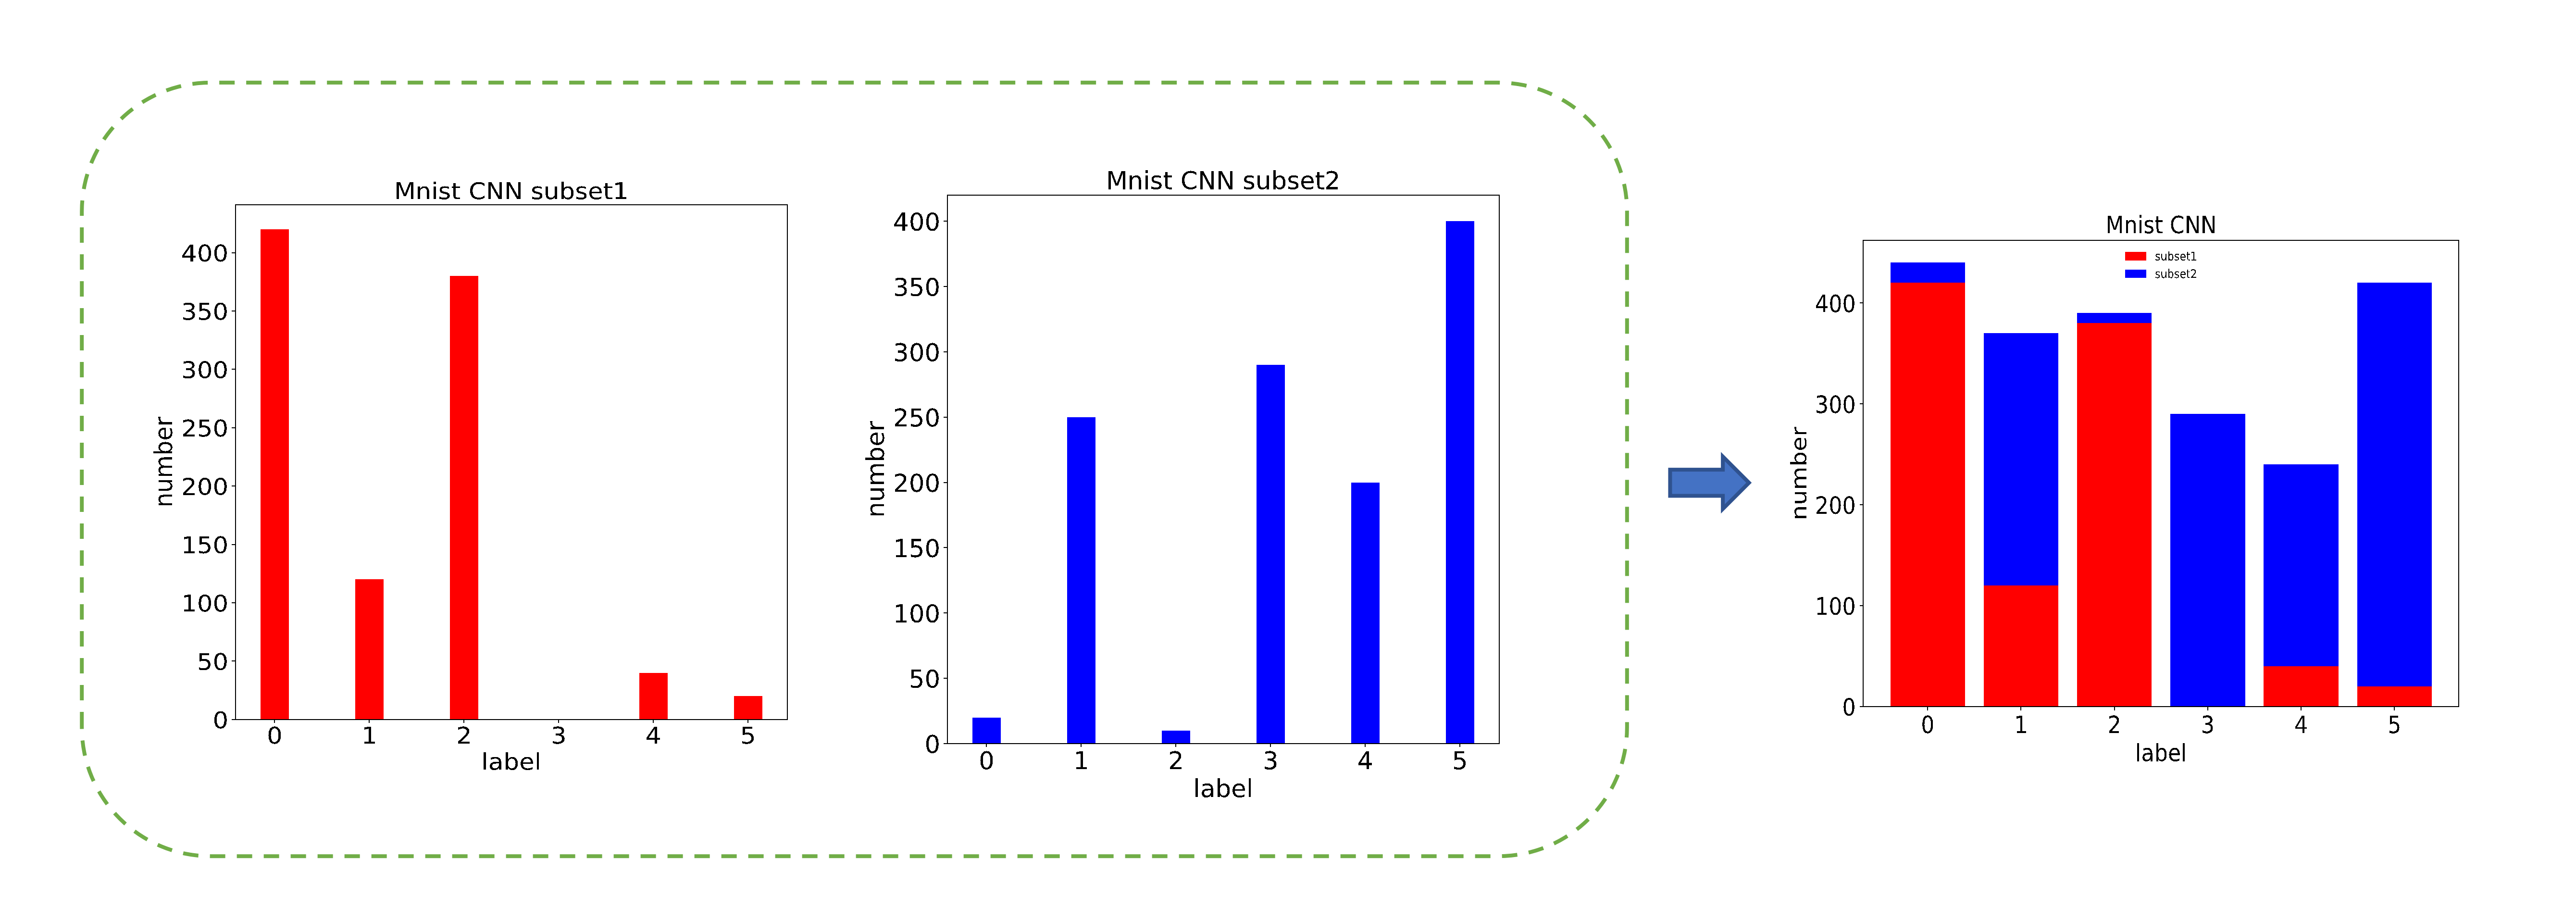
\includegraphics[width=5.5in]{fig9.png}
	\caption{Balanced sample distribution achieved under the complementarity of aggregated subsets.}
	\label{fig9}
\end{figure}
\vspace{-0.3cm}

% needed in second column of first page if using \IEEEpubid
%\IEEEpubidadjcol

\section{Loss-Based Algorithm Description}\label{section1.2}
Algorithm 1 shows the training process of the Loss-based screening strategy. During local training epoch $e$, in line 3, worker $k$ will check whether the query information is received. After receiving the query information from the parameter server, it indicates that the client has not completed the local update in the first stage of the timing query mechanism, and it is necessary to judge whether the update progress can be truncated in the current round to supplement the server. Client $k$ receives the aggregated subset model $\mathrm{w}_{\mathrm{r}}^{\mathrm{s}_{1}}$ of the first stage and then performs model inference based on the local dataset to obtain the loss and upload it to the server, in lines 3-5.  The server will sort the received loss in ascending order and wait for the client receiving top $N$ as supplementary clients. In lines 22-26, within the duration $T2$, for the selection of $N$, since the first-stage client and the second-stage client complement each other, we set the client scale in the two stages to a ratio of approximately 1:1 to avoid the imbalance in scale. 

\begin{algorithm}[!htbp] 
\caption{Loss-Based Screening Strategy} 
\begin{algorithmic}[1] %这个1 表示每一行都显示数字
\REQUIRE ~~\\ %算法的输入参数:Input
\STATE $w_{r-1}^{k}=w_{r}$
\FOR{ each local training epoch $e$ from 1 to $E$}
\IF{Receive $\mathrm{E}_{\mathrm{ctrl}}$ and $w_{r}^{s_{1}}$ from the server}
\IF{$\mathrm{e}>\mathrm{E}_{\mathrm{ctrl}} $}
\STATE Calculate $\operatorname{loss}_{k}$ by $\ell\left(x_{k}, w_{r}^{s_{1}}\right)$ and Upload  $\operatorname{loss}_{k}$
\IF{$\operatorname{loss}_{k}$ in top $N$}
\STATE Upload local model $w_{r}^{k}$
\RETURN
\ENDIF
\ENDIF
\ENDIF
\ENDFOR
\STATE Update local model
\STATE Upload local model $w_{r}^{k}$
\ENSURE ~~\\
\STATE $\mathcal{V}_{r}=\emptyset$, $\mathcal{L}_{r}=\emptyset$
\WHILE{$ use\_{time} < T1$}
\STATE Receive local model $w_{r}^{k}$ from client $c_{k}$
\STATE $\mathcal{V}_{r}=\mathcal{V}_{r} \cup\left\{c_{k}\right\}$
\ENDWHILE
\STATE Update global model $w_{r}^{s_{1}}$
\STATE Distribute \{ $\mathrm{E}_{\text {ctrl }, \mathrm{w}_{r}^{s_{1}}}$\} to the rest clients
\STATE Get $L_{r}=\left\{\operatorname{los} s_{1}, \operatorname{los} s_{2}, \ldots, \operatorname{loss}_{k}\right\}$ from the rest clients
\STATE Sort $L_{r}$ in ascending order and select the top $N$ clients
\WHILE{$ use\_{time} < T2$}
\STATE Receive local model $w_{r}^{k}$ from client $c_{k}$
\STATE $\mathcal{V}_{r}=\mathcal{V}_{r} \cup\left\{c_{k}\right\}$
\ENDWHILE
\STATE Update global model
\end{algorithmic}
\end{algorithm}

In terms of privacy protection, calculating the loss function is more complicated than calculating the EMD function. For example, the cross-loss function adds not only the logarithmic function operation but also the true label probability and the predicted label probability are unknown to the attacker, which increases the complexity of the attacker's reverse analysis. Therefore, it can be flexibly selected whether to combine secure multi-party computing or other privacy protection technologies to enhance privacy protection according to the computational complexity of the loss function. 

\section{Experimental Verification of Loss Indicator}\label{section1.3}
We use the handwritten digit recognition task of the Mnist dataset as an experimental scenario for experimental verification. The total number of clients is set to 100, the interaction round is set to 25, the local fixed iterative update round $E$ is set to 10, and the iteration round limit for truncated clients is 5. 

To verify the effect of the data distribution evaluation method based on the loss function in screening supplementary strategies, we selected the top $N$ method in the ascending order of the absolute value of the loss for experiments. We compared it with the method in descending order of the absolute value of the loss. That is, on the original rule of selecting a client with a larger loss, a rule for selecting a client with a smaller loss is set for experimental comparison to verify the effectiveness of the screening method.

In terms of comparative evaluation indicators, we selected two indicators: test accuracy and the aggregated subset size. The aggregated subset size is shown in \ref{12}.

\begin{equation}
\label{12}
	N_{\text {cluster }}=\frac{\sum_{r=1}^{R} \sum_{i=1}^{C} N(y=i)}{R}
\end{equation}

\noindent
where $N_{\text {cluster }}$ represents the average size of the aggregated subset, $R$ indicates the total number of interaction rounds, and $N(y=i)$ represents the number of samples of class $i$. Its statistical records are shown in figure \ref{fig10}. 

\begin{figure}[!htbp]
\vspace{-0.4cm} 
	\centering
	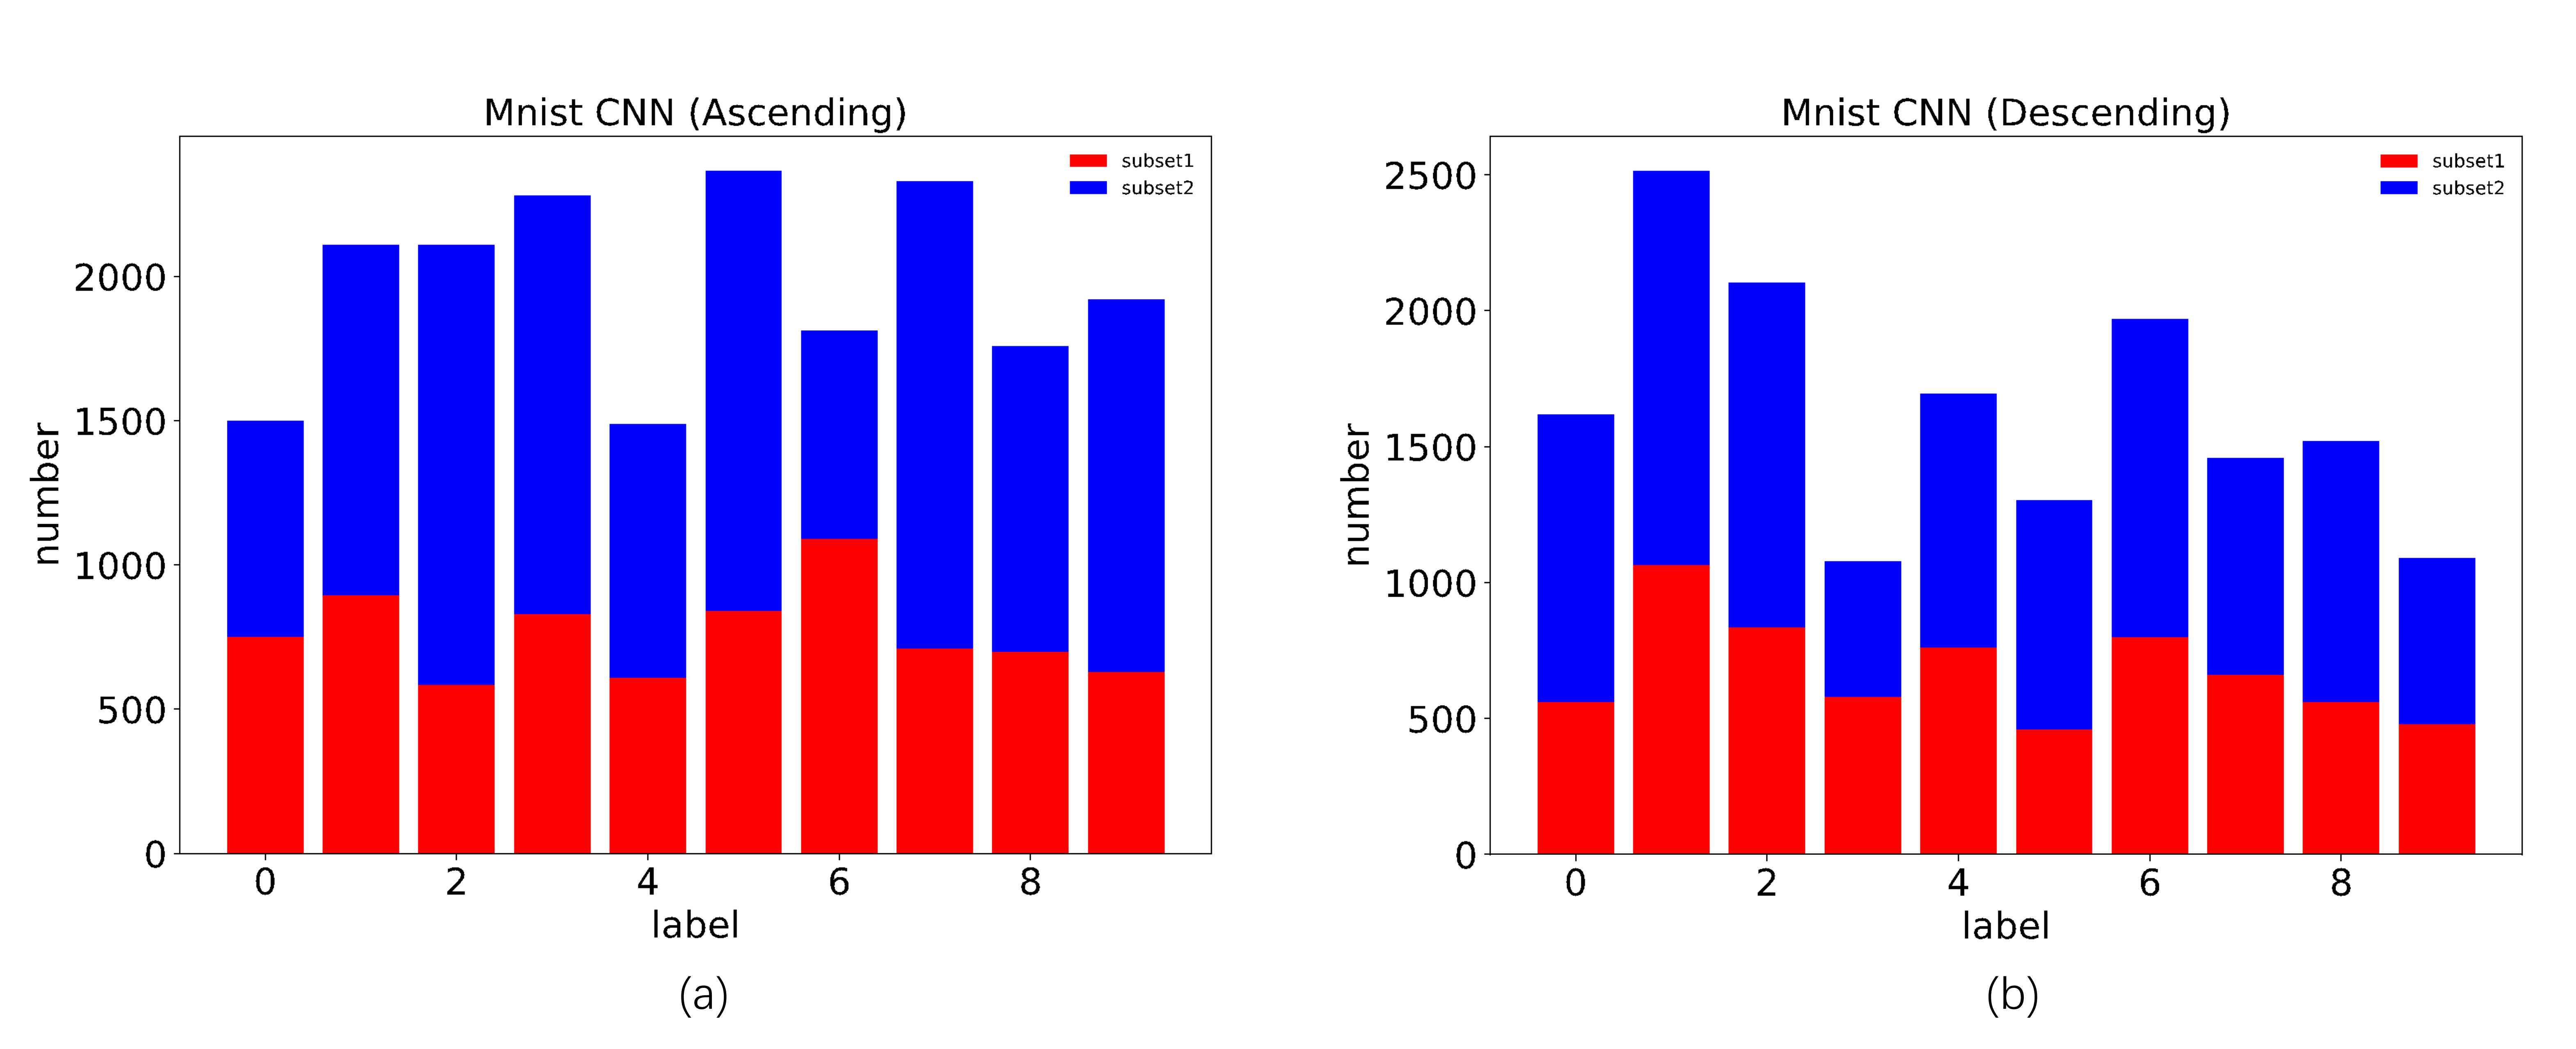
\includegraphics[width=5.5in]{fig10.png}
	\caption{Aggregated subset size under different loss screening supplementary strategies.}
	\label{fig10}
\end{figure}

Compared to figure \ref{fig10}, it can be found that in the descending loss screening strategy, for the aggregated subsets received in the timing query stage, the data samples of category 1, category 3 and category 6 occupy a large proportion, while the proportion of category 2, category 4 and category 9 is relatively small. After the truncated client is supplemented with it in the second stage, the proportion of category 6 in the sample combination in the first stage is controlled to a certain extent, and the proportion of category 2 and category 9 is gradually increased to approximate balance with category 1, so that the sample combination in the final aggregated subset reaches a more balanced state. 

Compared with the descending loss screening strategy, in the combination of the ascending loss screening strategy, for the aggregated subsets received in the timing query stage, the proportion of category 1, category 2 and category 6 is larger, while the proportion of category 3, category 5 and category 9 is relatively small. After the truncated supplementary clients in the second stage supplement it, the clients occupying a larger proportion and the clients occupying a smaller proportion still do not show a complementary effect with the proportional distribution of the first stage, but make the proportion of category 1 and category 6 still relatively high. 

It can be found that, when combined with the descending loss screening strategy, the sample data that has not been learned in the first-stage sample combination can be screened from the sample attributes and sample labels. Therefore, after screening and supplementing clients for uploading and supplementing, the distribution ratio of different samples in the sample combination can be controlled within a relatively balanced range. When combined with the ascending loss screening strategy, the screened clients contain more similar proportions of client sample combinations in the previous stage. Therefore, after the client is supplemented later, although the sample size is expanded, it fails to balance the sample combination and aggravates the imbalance between the proportions of different samples.

In addition, we recorded the test accuracy of the global model by combining the descending loss screening strategy and the ascending loss screening strategy, as shown in figure \ref{fig11}. First, in terms of convergence speed, the former begins to converge gradually around the 15th round and remains stable, while the test accuracy of the latter has always been presented in the form of oscillation, and it has never been able to converge. In terms of accuracy improvement, the former begins to increase to 0.90 and above after 7 interaction rounds, while the change curve of the latter not only improves slowly but also drops significantly when the interaction round is 7, which reflects the disturbance of the global aggregation model due to the imbalance of sample distribution. In terms of model performance, the test accuracy of the former converges to 0.9664, while the latter oscillates around 0.94, which cannot achieve stable convergence of model performance.  

\begin{figure}[!htbp]
\vspace{-0.4cm}
	\centering
	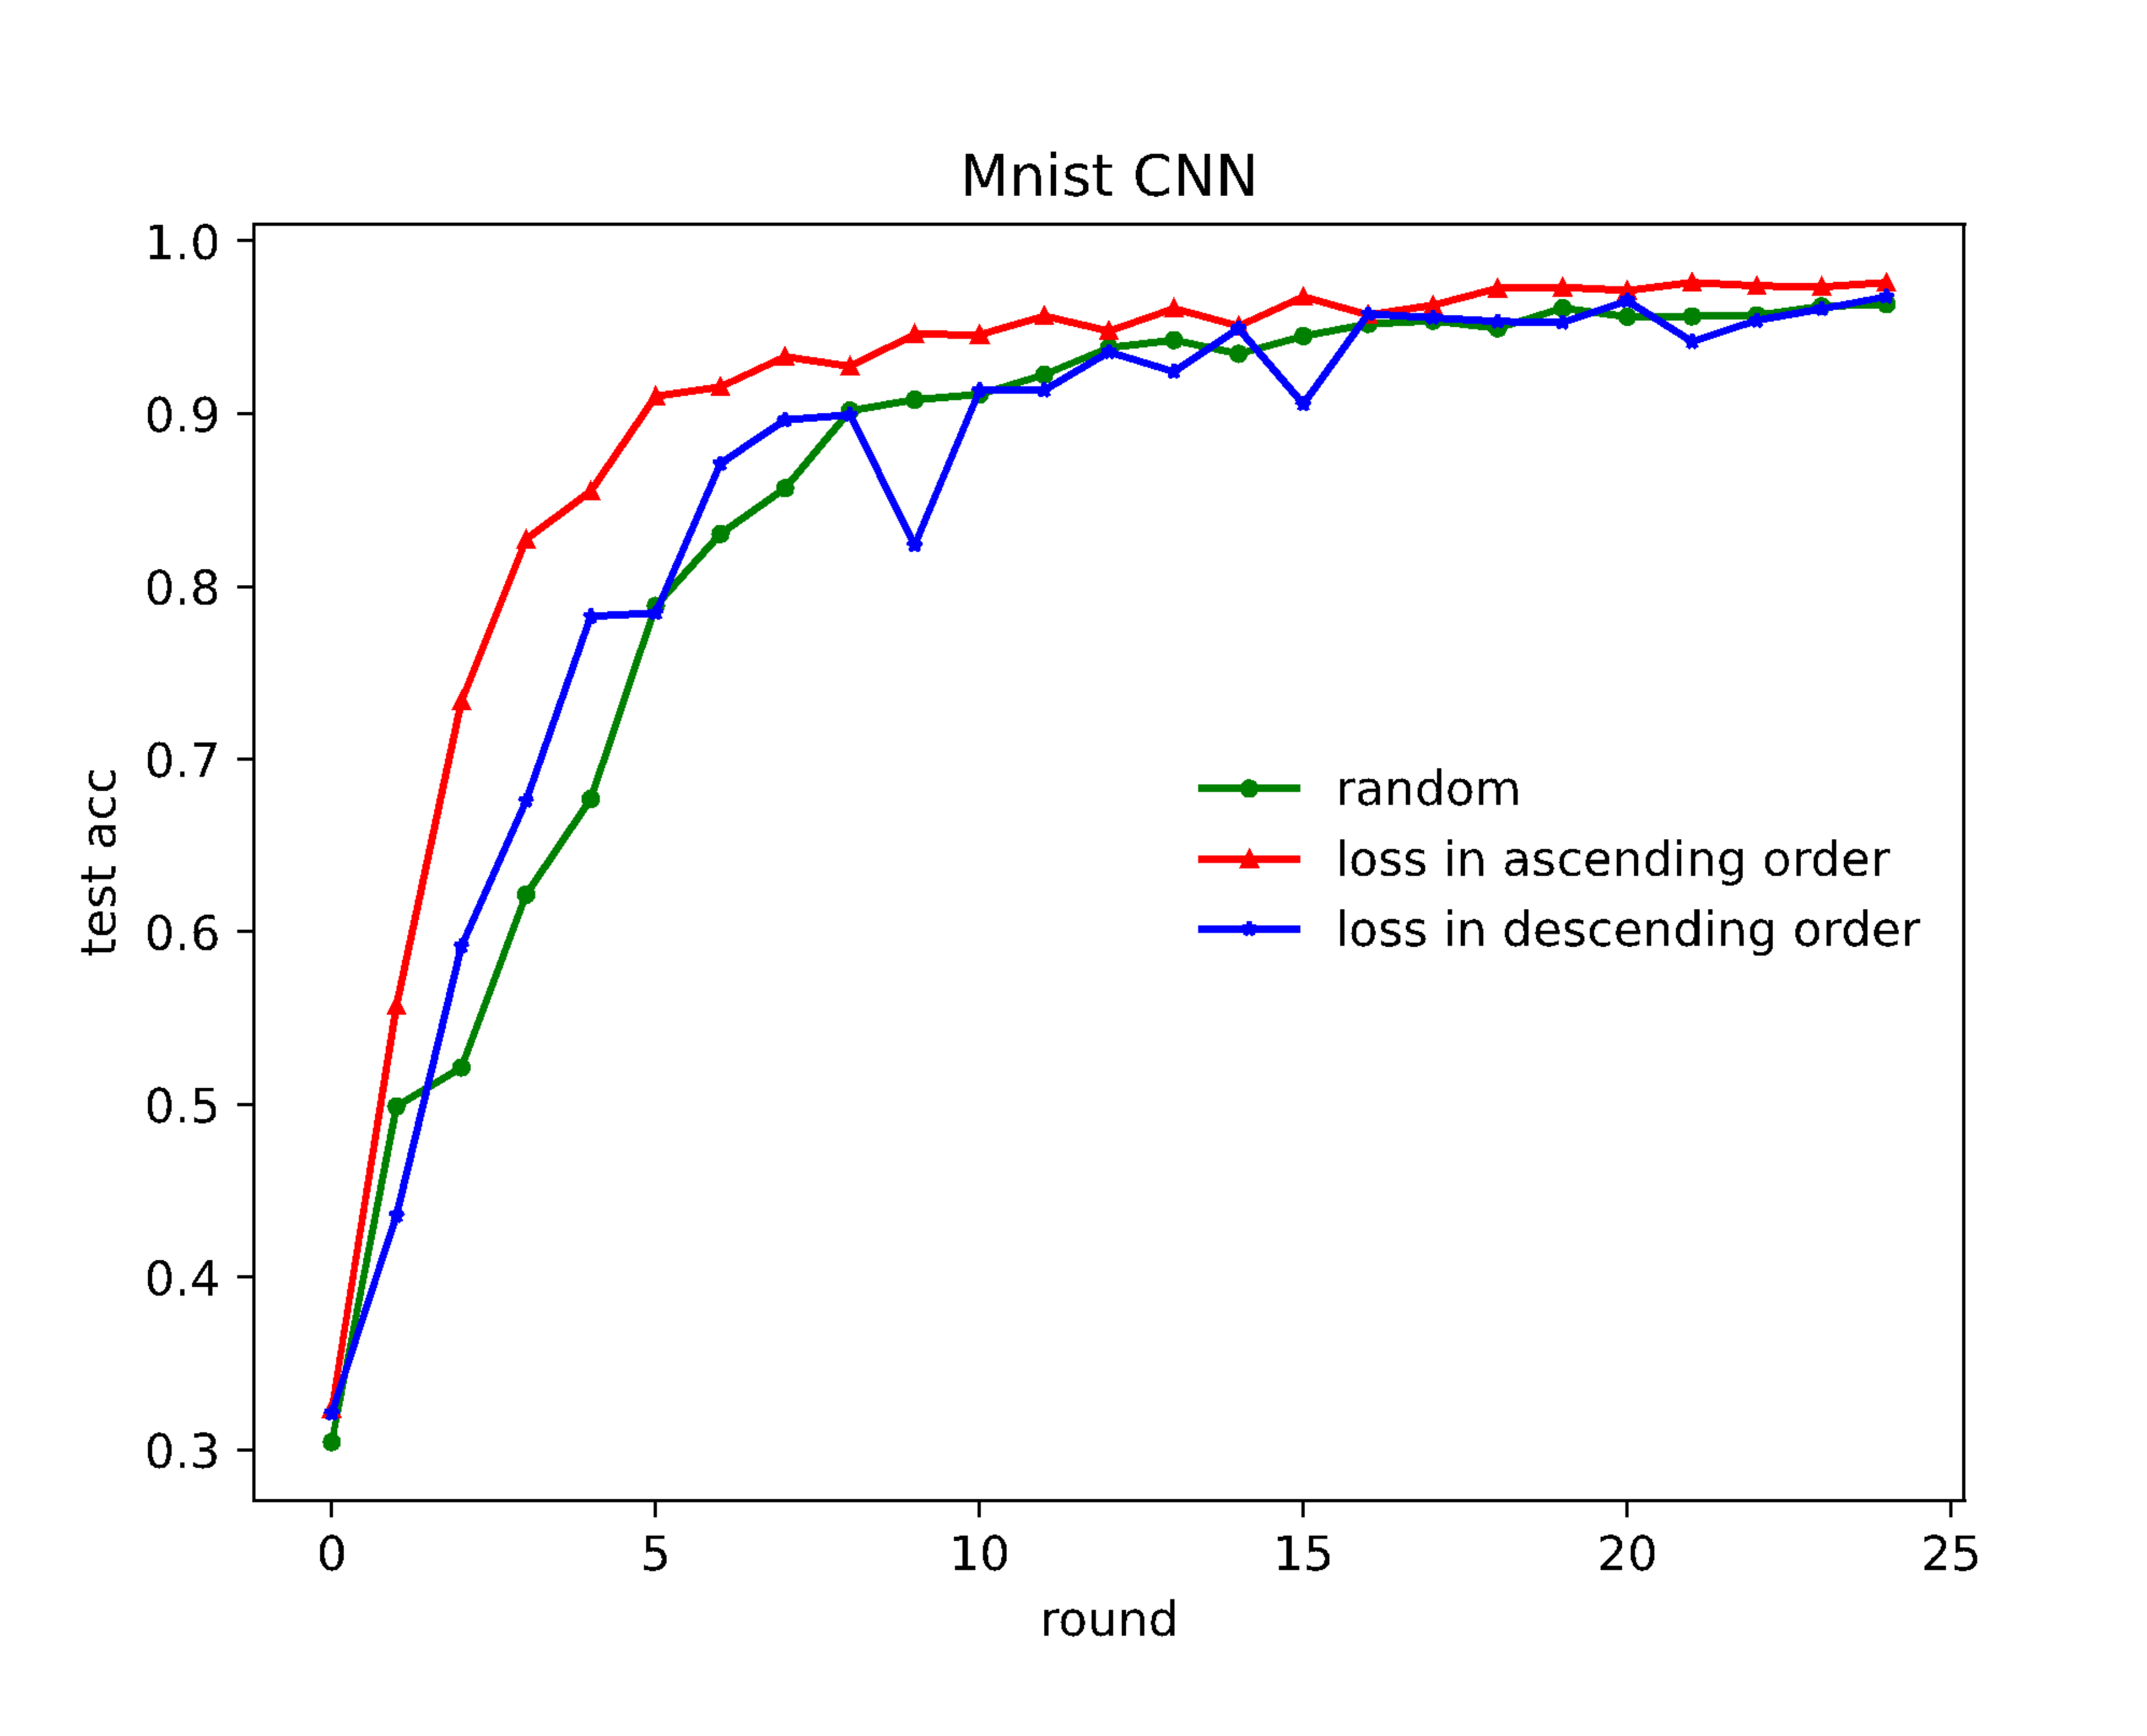
\includegraphics[width=0.6\linewidth]{fig11.png}
	\caption{Test accuracy different loss screening supplementary strategies.}
	\label{fig11}
\end{figure}

According to the above experimental verification and analysis, on the one hand, we can find that the unbalanced proportion of sample combinations has an adverse impact on the global aggregation model, which is not only reflected in the performance of the model but also dramatically interferes with the model training process of federated learning in terms of convergence speed and convergence stability. On the other hand, the aggregated subset model received in the first stage is used as the base classifier to evaluate the sample distribution of the remaining clients. The base classifier is controlled as an invariant, and the sample distribution of each remaining client is used as an independent variable. Different absolute values of the loss are used as dependent variables to sort and filter the remaining clients, thereby selecting a supplementary subset that is more suitable for the first-stage aggregated subset, which reflects the effectiveness of the screening supplementary strategy based on data distribution evaluation. Finally, in terms of different loss screening supplementary strategies, selecting clients with a larger loss is similar to magnifying error samples in the idea of Boosting algorithm, so that a sample set that is more complementary to the first-stage aggregated subset can be effectively selected. Clients with smaller loss represent a sample set that is similar to the first-stage aggregated subset, which cannot balance the final aggregated subset sample combination but makes the proportion of different samples more unbalanced. 

\section{Comparative Analysis Different Screening Indicators}\label{section1.4}

From the above, we propose two screening supplementary strategies, E-FedTS and L-FedTS, based on two different screening indicators, EMD and Loss. The differences between the two are as follows.

(1) There are differences in the query information between the two. When the parameter server sends the query information, in addition to the iteration round limit information, the E-FedTS needs to send the EMD calculation information of the first stage. The L-FedTS needs to send the aggregated model information of the first stage.

(2) The two are different in the comparison and screening method of the client. The EMD information in the E-FedTS protocol is a simple calculation of the label distribution skewness in the local dataset. The L-FedTS uses the global aggregated model of the first stage as the base classifier and performs model inference on the local dataset to obtain the loss degree of the local dataset in the remaining clients.

(3) Since the two have different query information, when the parameter server sends the query information to the remaining clients, the delivery time occupied by the parameter server on the communication link will also be different. In the E-FedTS, we set the EMD indicator as 4-byte floating-point data. The L-FedTS needs to send the aggregated model parameters of the first stage as the base classifier of the current round to the remaining clients. Some studies can constrain the lightweight model in federated learning to about 20Mb \cite{zhang2011m}, \cite{zhang2015simulation}. Therefore, the L-FedTS has a higher communication cost than the E-FedTS. With the optimization and improvement of the broadband network, the download speed has been greatly improved compared with the upload speed, such as Gigabit network, 2.5G network and portable wifi. For the broadband of the Gigabit network, since one byte has eight bits, its download speed can theoretically reach 1000Mbps/8=125Mb/s, and it can be close to 100Mb/s under a certain loss. From this, it can be concluded that the download time of EMD indicator information can be ignored, and the download time under the L-FedTS can be controlled at about 0.2s. Therefore, when sending the query information, the L-FedTS takes about 0.2s more time than the E-FedTS.

(4) In comparing and screening clients, after the L-FedTS client receives the base classifier, the remaining clients need to perform model inference based on the local dataset. Raspberry Pi is a common experimental device in edge computing. To better analyze the inference time of the model on this device, a study \cite{zhang2021adaptive} found that by splitting the model by network layer and recording its inference time, the inference time of different network layers of the model on the Raspberry Pi is independent of the memory occupied by the network layers. Among them, the inference time of the convolutional neural network layer fluctuates in the range of [50ms, 1300ms], which is the network layer that occupies the longest inference time in the entire model, while other network layers mainly fluctuate in the range of [10ms, 50ms]. Therefore, for the model under the handwritten character recognition task in this paper, since the inference time occupied by multiple interaction rounds is different, if we assume that the average inference time in multiple interaction rounds is 500ms, compared with the E-FedTS, the L-FedTS has about 0.5s more waiting time when the client performs screening evaluation.

(5) Finally, the convergence rate in the global aggregated model’s update process and the model performance’s improvement effect are analyzed. We take the handwritten digit recognition task of the Mnist dataset as the experimental scene, set the ratio of fast, medium and slow clients to 3: 4: 3, the total number of clients is set to 100, and the number of interaction rounds is set to 25. The local fixed iterative update round E is set to 10, and the iteration round limit of the truncated client is 5. The model performance records of the two in the global model update process are shown in figure \ref{fig12}. The E-FedTS and the L-FedTS have improved the global aggregated model performance and the convergence rate, but the optimization effect of the L-FedTS is higher than that of the E-FedTS. 

\begin{figure}[!htbp]
\vspace{-0.4cm} 
	\centering
	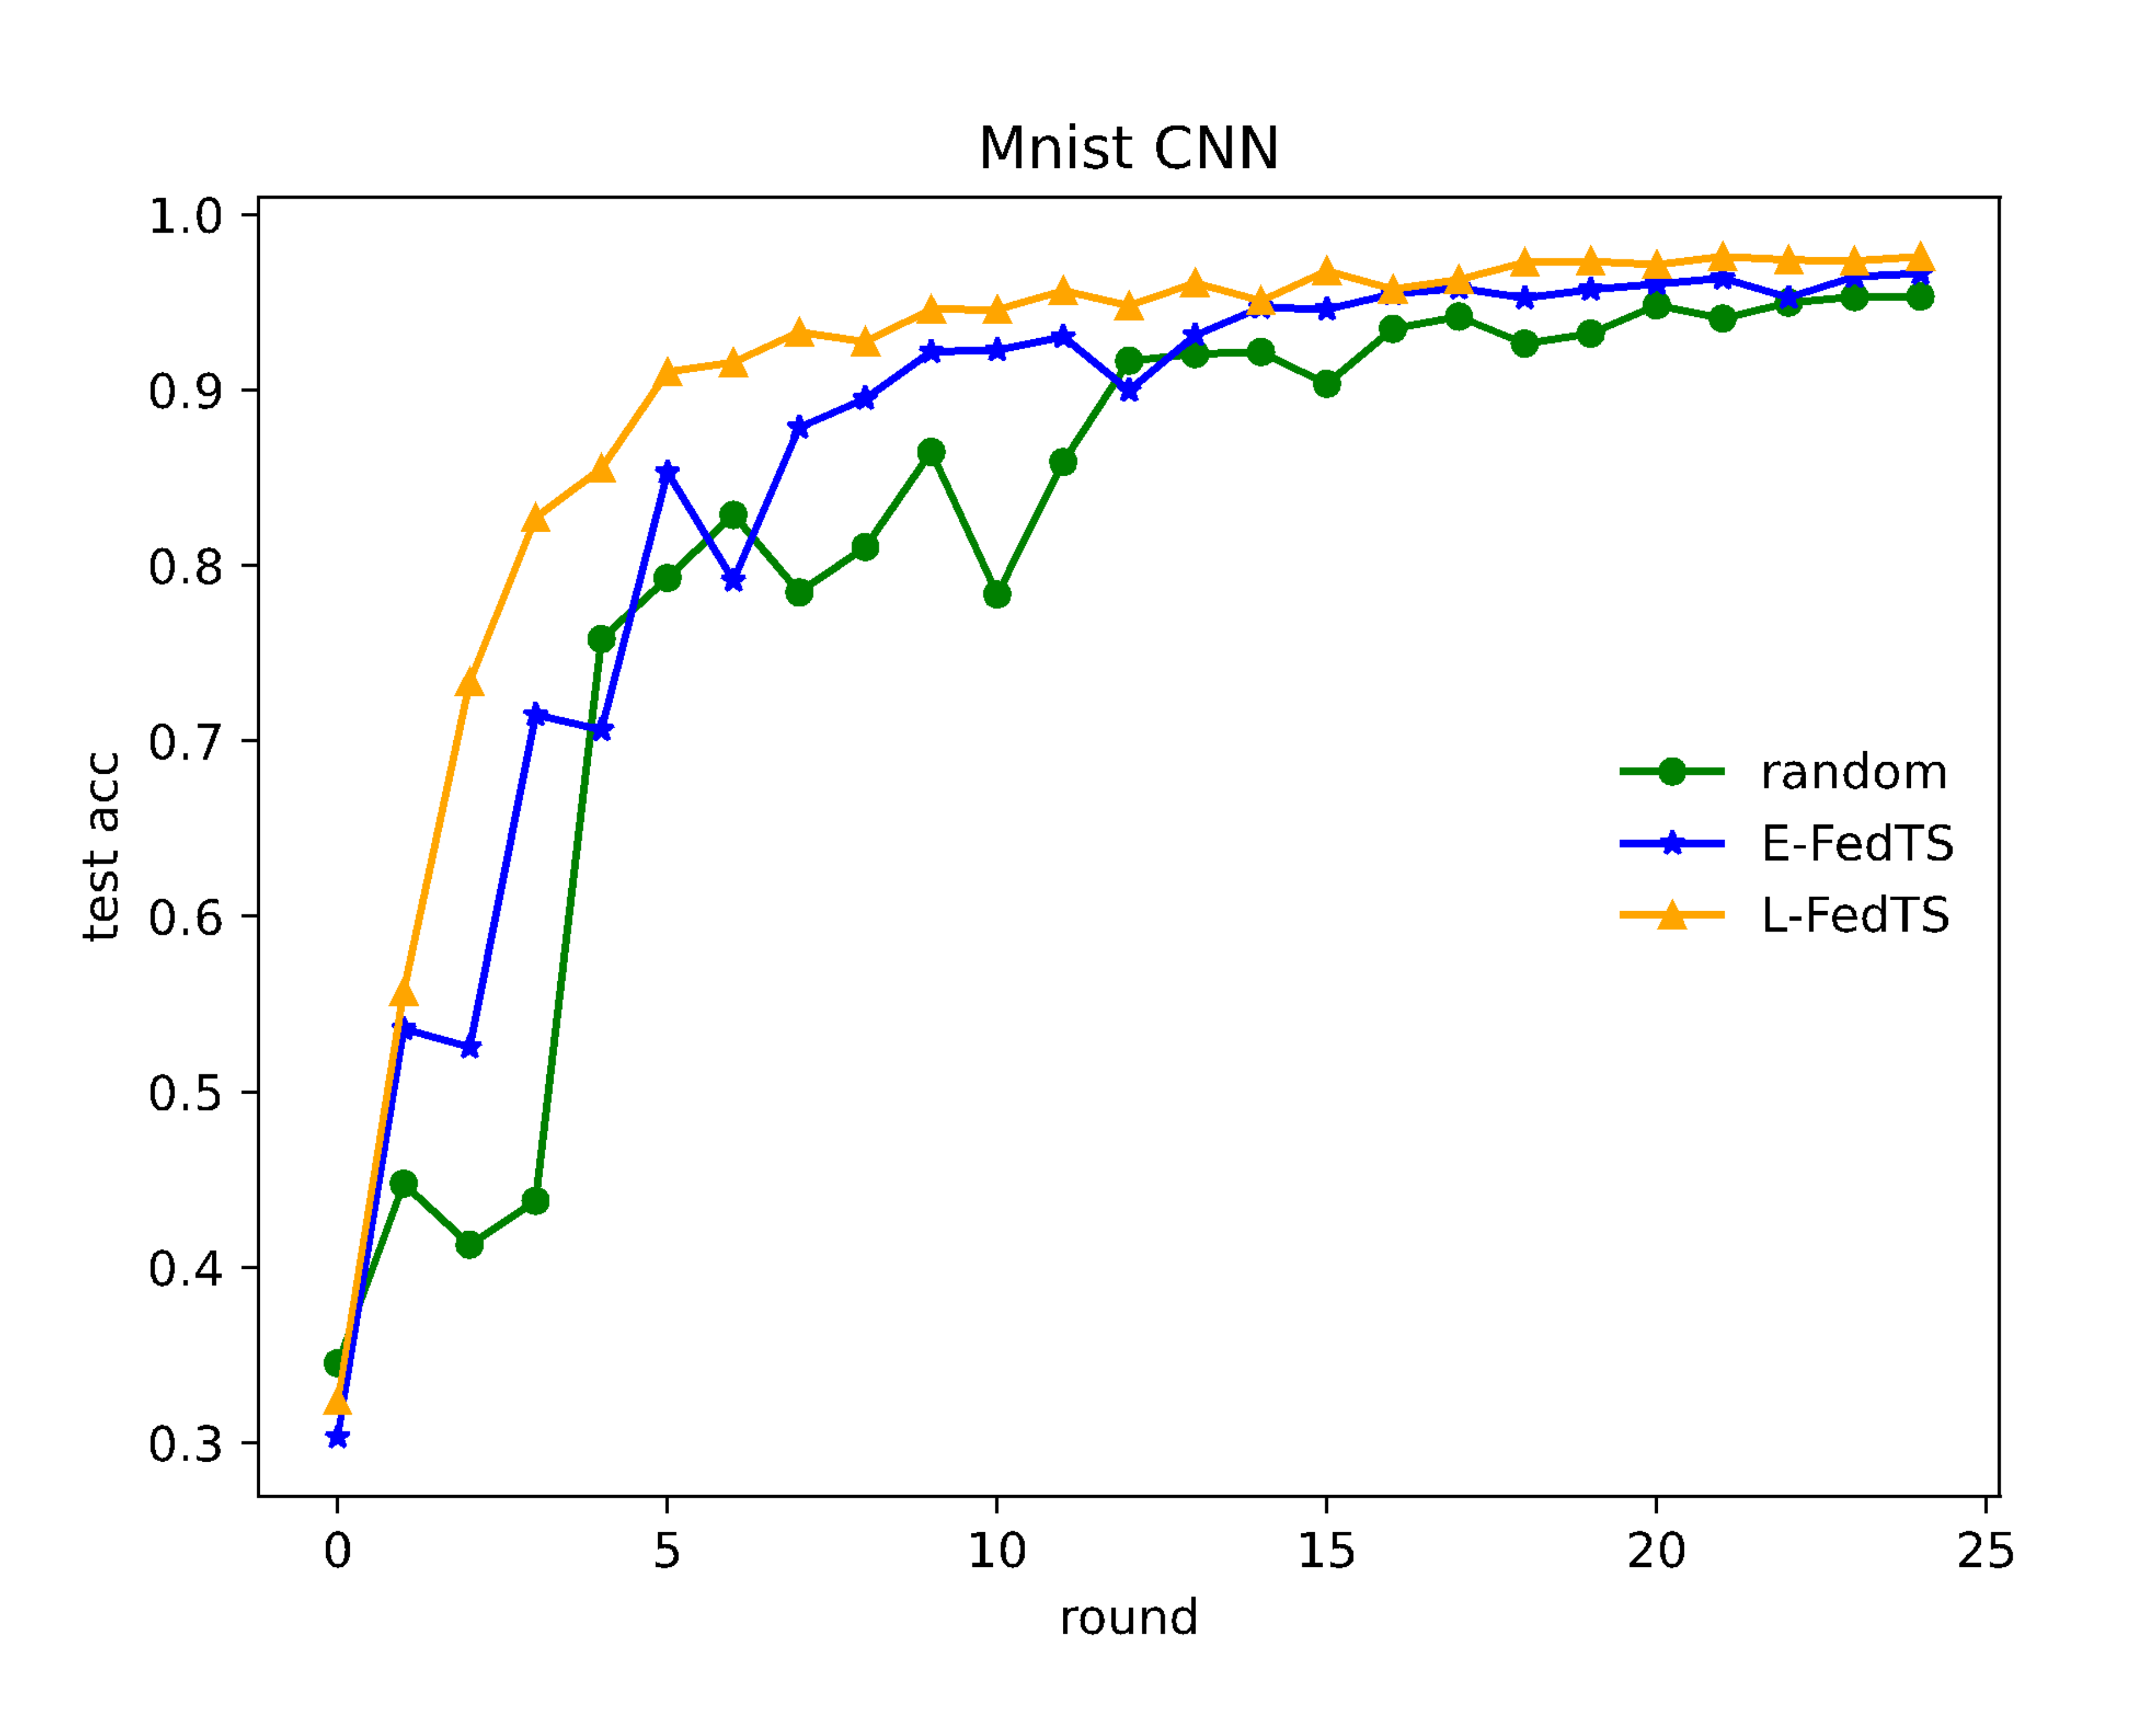
\includegraphics[width=0.6\linewidth]{fig12.png}
	\caption{Global model performance under different screening supplementary strategies.}
	\label{fig12}
\end{figure}

It can be seen from the above analysis that the improvement effect of the L-FedTS is more evident than that of the E-FedTS, but the duration is also more than that of the E-FedTS protocol. Therefore, we can choose which screening strategy is more suitable according to different needs and client performance.

\section{Conclusion}
In this paper we introduce a Federated learning protocol for edge devices base on loss indicator,incorporating a timing query mechanism and screening supplementary strategies.We analyze loss indicator and design Loss-Based algorithm.Through experimental verification of loss indicator and comparative analysis of different screening indicators,L-fedTS ensures the efficiency of federated learning in terms of interaction efficiency and convergence efficiency. 
















\bibliographystyle{unsrtnat}
\bibliography{references}  %%% Uncomment this line and comment out the ``thebibliography'' section below to use the external .bib file (using bibtex) .


%%% Uncomment this section and comment out the \bibliography{references} line above to use inline references.
% \begin{thebibliography}{1}

% 	\bibitem{kour2014real}
% 	George Kour and Raid Saabne.
% 	\newblock Real-time segmentation of on-line handwritten arabic script.
% 	\newblock In {\em Frontiers in Handwriting Recognition (ICFHR), 2014 14th
% 			International Conference on}, pages 417--422. IEEE, 2014.

% 	\bibitem{kour2014fast}
% 	George Kour and Raid Saabne.
% 	\newblock Fast classification of handwritten on-line arabic characters.
% 	\newblock In {\em Soft Computing and Pattern Recognition (SoCPaR), 2014 6th
% 			International Conference of}, pages 312--318. IEEE, 2014.

% 	\bibitem{hadash2018estimate}
% 	Guy Hadash, Einat Kermany, Boaz Carmeli, Ofer Lavi, George Kour, and Alon
% 	Jacovi.
% 	\newblock Estimate and replace: A novel approach to integrating deep neural
% 	networks with existing applications.
% 	\newblock {\em arXiv preprint arXiv:1804.09028}, 2018.

% \end{thebibliography}


\end{document}
